\section{Quantum circuits}

In the previous chapter, we discussed the classical models of computation including classical circuits. In this chapter, we will discuss about the quantum circuits which lie at the heart of quantum computation. There are two main ideas introduced in this chapter. First, we explain in detail the fundamental model of quantum computation, the quantum circuit model. Second, we demonstrate that there exists a small set of gates which are \textit{universal}, that is, any quantum computation whatsoever can be expressed in terms of those gates.

\subsection{Single qubit operations}

As we have already seen previously that a qubit is a vector $\ket{\psi} = a\ket{0} + b\ket{1}$ parameterized by two complex numbers satisfying $|a|^2 + |b|^2 = 1$. Operations on a qubit must preserve this norm, and thus are described by $2 \times 2$ unitary matrices. It should be noted that \textit{all} unitary matrices are valid gates for a qubit. Here are some commonly used single qubit gates: 
\begin{figure}[h]
    \centering
    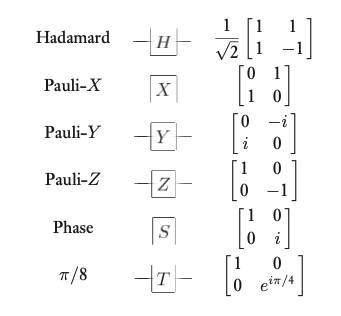
\includegraphics[width=0.45\textwidth]{gates.png}
    \caption{Names, symbols, and unitary matrices for the common single qubit gates.}
\end{figure}
\vspace{1em}

\subsection{Controlled operations}

'If A is true, then do B'. This type of \textit{controlled operation} is one of the most useful in computing, both classical and quantum.
\vspace{1em}

Suppose we have a single qubit gate $U$. A \textit{Controlled-$U$} gate is a two qubit gate which takes in an extra qubit called control qubit which is either $\ket{0}$ or $\ket{1}$. If it is $\ket{1}$, then the gate $U$ is applied on the other qubit (target qubit). However, if it is $\ket{0}$, then the other qubit is not changed. Mathematically, $\ket{c}\ket{t} \rightarrow \ket{c}U^c\ket{t}$ where $U^c = U$ if $c = \ket{1}$ and $U^c = I$ if $c = \ket{0}$. It is represented as follows.
\begin{figure}[h]
    \centering
    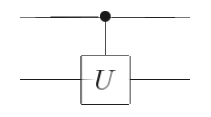
\includegraphics[width=0.20\textwidth]{controlled.png}
    \caption{Controlled-$U$ operation}
\end{figure}
\vspace{1em}

If $U$ is the NOT gate, then we get what is called the CNOT gate. It is a very useful gate as we will see later and has the following matrix representation.

$$\begin{bmatrix}
1&0&0&0\\
0&1&0&0\\
0&0&0&1\\
0&0&1&0\\
\end{bmatrix}$$
\vspace{1em}

The advantage of CNOT gate that any general controlled-$U$ gate can easily be derived CNOT gate by using the circuit given below.
\begin{figure}[h]
    \centering
    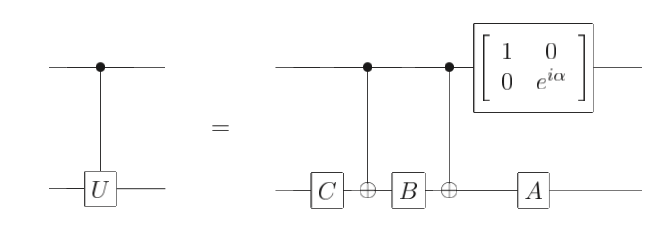
\includegraphics[width=0.70\textwidth]{cu.png}
    \caption{Circuit implementing the controlled-$U$ operation for single qubit gate $U$. $\alpha$, $A$, $B$ and $C$ satisfy $U = e^{i\alpha}A\times B\times C$, $ABC = I$.}
\end{figure}
\vspace{1em}

\subsection{Measurement}

A final element used in quantum circuits, almost implicitly sometimes, is measurement. In circuit diagrams, a measurement is reresented using the 'meter' symbol. In the theory of quantum circuits it is conventional to not use any special symbols to denote more general measurements, because they can always be represented by unitary transforms with ancilla qubits followed by projective measurements.
\vspace{1em}
\begin{figure}[h]
    \centering
    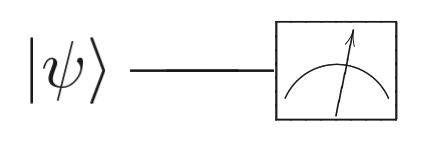
\includegraphics[width=0.40\textwidth]{meter.png}
    \caption{Symbol for measurement on a single qubit.}
\end{figure}
\vspace{1em}

There are two important principles that it is worth bearing in mind about quantum circuits.

\begin{enumerate}
    \item\textbf{Principle of deferred measurement}: Measurements can always be moved from an intermediate stage of a quantum circuit to the end of the circuit; if the measurement results are used at any stage of the circuit then the classically controlled operations can be replaced by conditional quantum operations.
    \item\textbf{Principle of implicit measurement}: Without loss of generality, any unterminated quantum wires (qubits which are not measured) at the end of a quantum circuit may be assumed to be measured.
\end{enumerate}

\subsection{Universal quantum gates}

A set of gates is said to be universal for quantum computation if any unitary operation may be approximated to arbitrary accuracy by a quantum circuit involving only those gates.
\vspace{1em}

We now describe three universality constructions for quantum computation.

\subsubsection{Two-level unitary gates are universal}

Consider a unitary matrix $U$ which acts on a $d$-dimensional Hilbert space. In this section we explain how $U$ may be decomposed into a product of two-level unitary matrices; that is, unitary matrices which act non-trivially only on two-or-fewer vector components. The essential idea behind this decomposition may be understood by considering the case when $U$ is $3\times 3$, so suppose that $U$ has the form
$$U = \begin{bmatrix}
a&d&g\\
b&e&h\\
c&f&j
\end{bmatrix}$$

We will find two-level unitary matrices $U_1, U_2, U_3$ such that
$$U_3U_2U_1U = I$$
It follows that
$$U = U_1^\dag U_2^\dag U_3^\dag$$

$U_1$, $U_2$ and $U_3$ are all two-level unitary matrices, and it is easy to see that their inverses, $U_1^\dag$, $U_2^\dag$ and $U_3^\dag$ are also two-level unitary matrices.
\vspace{1em}

Use the following procedure to construct $U_1$: if $b = 0$ then set
$$U_1 \equiv \begin{bmatrix}1&0&0\\0&1&0\\0&0&1\end{bmatrix}$$
If $b \neq 0$ then set
$$U_1 \equiv \begin{bmatrix}
\frac{a^\ast}{\sqrt{|a|^2+|b|^2}} & \frac{b^\ast}{\sqrt{|a|^2+|b|^2}} &0\\
\frac{b}{\sqrt{|a|^2+|b|^2}} & \frac{-a}{\sqrt{|a|^2+|b|^2}} &0\\
0&0&1
\end{bmatrix}$$

Note that in either case $U_1$ is a two-level unitary matrix, and when we multiply the matrices out we get
$$U_1U = \begin{bmatrix}
a'&d'&g'\\
0&e'&h'\\
c'&f'&j'
\end{bmatrix}$$

The key point to note is that the middle entry in the left hand column is zero. Now apply a similar procedure to find a two-level matrix $U_2$ such that $U_2U_1U$ has no entry in the bottom left corner. That is, if $c' = 0$ we set
$$U_2 \equiv \begin{bmatrix}a'^\ast&0&0\\0&1&0\\0&0&1\end{bmatrix}$$
while if $c' \neq 0$ then we set
$$U_2 \equiv \begin{bmatrix}
\frac{a'^\ast}{\sqrt{|a'|^2+|c'|^2}} &0& \frac{a'^\ast}{\sqrt{|a'|^2+|c'|^2}}\\
0&1&0\\
\frac{c'}{\sqrt{|a'|^2+|c'|^2}} &0& \frac{-a'}{\sqrt{|a'|^2+|c'|^2}}
\end{bmatrix}$$
In either case, when we carry out the matrix multiplication we find that
$$U_2U_1U = \begin{bmatrix}
1&d''&g''\\
0&e''&h''\\
0&f''&j''
\end{bmatrix}$$
Since $U$, $U_1$ and $U_2$ are unitary, it follows that $U_2U_1U$ is unitary, and thus $d'' = g'' = 0$ since the first row of $U_2U_1U$ must have norm $1$. Finally, set
$$U_3 = \begin{bmatrix}
1&0&0\\
0&e''^\ast&h''^\ast\\
0&f''^\ast&j''^\ast
\end{bmatrix}$$
It is now easy to verify that $U_3U_2U_1U = I$, and thus $U = U_1^\dag U_2^\dag U_3^\dag$, which is a decomposition of $U$ into two-level unitaries.
\vspace{1em}

More generally, suppose $U$ acts on a $d$-dimensional space. Then, in a similar fashion to the $3\times 3$ case, we can find two-level unitary matrices $U_1, \dots , U_{d-1}$ such that the matrix $U_{d-1}U_{d-2}\dots U_1U$ has a one in the top left hand corner, and all zeroes elsewhere in the first row and column. We then repeat this procedure for the $d - 1$ by $d - 1$ unitary submatrix in the lower right hand corner of $U_{d-1}U_{d-2}\dots U_1U$ , and so on, with the end result that an arbitrary $d\times d$ unitary matrix may be written
$$U = V_1\dots V_k$$
where the matrices $V_i$ are two-level unitary matrices, and $k \leq (d - 1) + (d - 2) + \dots + 1 = d(d-1)/2$.

\subsubsection{Single qubit and CNOT gates are universal}

Suppose $U$ is a two-level unitary matrix on an $n$ qubit quantum computer. Suppose
in particular that $U$ acts non-trivially on the space spanned by the computational basis
states $\ket{s}$ and $\ket{t}$, where $s = s_1\dots s_n$ and $t = t_1\dots t_n$ are the binary expansions for $s$ and $t$. Let $\widetilde{U}$ be the non-trivial $2\times 2$ unitary submatrix of $U$; $\widetilde{U}$ can be thought of as a unitary operator on a single qubit.
\vspace{1em}

Our immediate goal is to construct a circuit implementing $U$, built from single qubit and CNOT gates. To do this, we need to make use of \textit{Gray codes}. Suppose we have distinct binary numbers, $s$ and $t$. A Gray code connecting $s$ and $t$ is a sequence of binary numbers, starting with $s$ and concluding with $t$, such that adjacent members of the list differ in exactly one bit. For instance, with $s = 101001$ and $t = 110011$ we have the Gray code
$$\begin{matrix}1&0&1&0&0&1\\1&0&1&0&1&1\\1&0&0&0&1&1\\1&1&0&0&1&1\end{matrix}$$

Let $g_1$ through gm be the elements of a Gray code connecting $s$ and $t$, with $g_1 = s$ and $g_m = t$. Note that we can always find a Gray code such that $m \le n+1$ since $s$ and $t$ can differ in at most $n$ locations.
\vspace{1em}

Now, the first step is to swap the states $\ket{g_1}$ and $\ket{g_2}$. Suppose $g_1$ and $g_2$ differ at the $i$th digit. Then we accomplish the swap by performing a controlled bit flip on the $i$th qubit, conditional on the values of the other qubits being identical to those in both $g_1$ and $g_2$. Next we use a controlled operation to swap $\ket{g_2}$ and $\ket{g_3}$. We continue in this fashion until we swap $\ket{g_{m-2}}$ with $\ket{g_{m-1}}$. The effect of this sequence of $m − 2$ operations is to achieve the operation
\begin{equation*}
\begin{split}
    \ket{g_1} &\rightarrow \ket{g_{m-1}}\\
    \ket{g_2} &\rightarrow \ket{g_1}\\
    \ket{g_3} &\rightarrow \ket{g_2}\\
    &\dots\\
    \ket{g_{m-1}} &\rightarrow \ket{g_{m-2}}
\end{split}
\end{equation*}

All other computational basis states are left unchanged by this sequence of operations.
Next, suppose $g_{m−1}$ and $g_m$ differ in the $j$th bit. We apply a controlled-$\widetilde{U}$ operation with the $j$th qubit as target, conditional on the other qubits having the same values as appear in both $g_m$ and $g_{m−1}$. Finally, we complete the $U$ operation by undoing the swap operations: we swap $\ket{g_{m-1}}$ with $\ket{g_{m-2}}$, then $\ket{g_{m-2}}$ with $\ket{g_{m-3}}$ and so on, until we swap $\ket{g_2}$ with $\ket{g_1}$.
\vspace{1em}

We see that implementing the two-level unitary operation $U$ requires at most $2(n−1)$ controlled operations to swap $\ket{g_1}$ with $\ket{g_{m-1}}$ and then back
again. Each of these controlled operations can be realized using $O(n)$ single qubit and CNOT gates; the controlled-$\widetilde{U}$ operation also requires $O(n)$ gates. Thus, implementing $U$ requires $O(n^2)$ single qubit and CNOT gates. We saw in the previous section that an arbitrary unitary matrix on the $2n$-dimensional state space of $n$ qubits may be written as a product of $O(2^{2n}) = O(4^n)$ two-level unitary operations. Combining these results, we see that an arbitrary unitary operation on $n$ qubits can be implemented using a circuit containing $O(n^2 4^n)$ single qubit and CNOT gates. 
